%%%%%%%%%%%%%%%%%%%%%%%%%%%%%%%%%%%%%%%%%
% University/School Laboratory Report
% LaTeX Template
% Version 3.1 (25/3/14)
%
% This template has been downloaded from:
% http://www.LaTeXTemplates.com
%
% Original author:
% Linux and Unix Users Group at Virginia Tech Wiki 
% (https://vtluug.org/wiki/Example_LaTeX_chem_lab_report)
%
% License:
% CC BY-NC-SA 3.0 (http://creativecommons.org/licenses/by-nc-sa/3.0/)
%
%%%%%%%%%%%%%%%%%%%%%%%%%%%%%%%%%%%%%%%%%

%----------------------------------------------------------------------------------------
%	PACKAGES AND DOCUMENT CONFIGURATIONS
%----------------------------------------------------------------------------------------

\documentclass{article}

\usepackage[version=3]{mhchem} % Package for chemical equation typesetting
\usepackage{siunitx} % Provides the \SI{}{} and \si{} command for typesetting SI units
\usepackage{graphicx} % Required for the inclusion of images
\usepackage{natbib} % Required to change bibliography style to APA
\usepackage{amsmath} % Required for some math elements 
\usepackage[utf8]{inputenc} % slovenski znaki
\usepackage[]{algorithm2e}
\usepackage{hyperref}
\setlength\parindent{0pt} % Removes all indentation from paragraphs

\renewcommand{\labelenumi}{\alph{enumi}.} % Make numbering in the enumerate environment by letter rather than number (e.g. section 6)

%\usepackage{times} % Uncomment to use the Times New Roman font

%----------------------------------------------------------------------------------------
%	DOCUMENT INFORMATION
%----------------------------------------------------------------------------------------

\title{Letters} % Title

\author{Rok Koleša, Domen Kren, Darko Janković} % Author name

\date{\today} % Date for the report

\begin{document}

\maketitle % Insert the title, author and date

\begin{center}
Mentor: prof. dr. Neža Mramor Kosta % Instructor/supervisor
\end{center}

% If you wish to include an abstract, uncomment the lines below
% \begin{abstract}
% Abstract text
% \end{abstract}

\newpage
\tableofcontents
\newpage
%----------------------------------------------------------------------------------------
%	SECTION 1
%----------------------------------------------------------------------------------------

\section{Goal}
  Determine which capital letter is represented by given simplicial complex from the set of 12 letters of Slovenian alphabet. Simplicial complex is represented with a list of edges which consist of pairs of start and end points. Each point is given by a pair of coordinates.


\subsection{Definitions}
\label{definicije}
\begin{description}
\item[Vietoris–Rips complex] is an abstract simplicial complex that can be defined from any metric space $M$ and distance $r$ by forming a simplex for every finite set of points that has diameter at most $r$.
\item[Persistent homology] is a method for computing topological features of a space at different spatial resolutions.
\end{description} 
 
%----------------------------------------------------------------------------------------
%	SECTION 2
%----------------------------------------------------------------------------------------

\section{Input}
Images of letters, transformed into 1-dimensional simplicial complexes are in the files
a.png, b.png, ... , l.png
Images of the resulting simplicial complexes (so that you can see what they look like) are
in t\_a.png, t\_b.png, ... , t\_l.png
Triangulations of the letters: a.out, b.out, ... , l.out
Each file contains only edges which are given as a list of two points: the starting point
and the ending point of the edge. Each point is given by a pair of coordinates.

%----------------------------------------------------------------------------------------
%	SECTION 3
%----------------------------------------------------------------------------------------

\section{Solution}
As seen in our goal specification, we tackled this problem of letter classification with persistent homology. 
The main idea of our solution is looking at different parts of objects and computing their homologies. The 
algorithm is divided into three parts:

\begin{enumerate}
\item First, let us parse the input. All we need is a set of points that are part of the object we want to classify. The
only problem that can arise, comes from the distribution of the points. If they are all in one place or to sparse, we
will not be able to get good results. We want an even distribution with lots of points.

\item We slowly ''sink'' our letter. After sorting our input points we cut the letter by layers. After that we compute 
homologies for each of those. 

For the computations, we compute the Vietoris-Rips complex and intervals and check infinite ones. With that we can get the number of components and cycles in our complex.
We have to be a little careful with how we choose the maximum radius value, for the Vietoris-Rips algorithm. With some
trial and error we decided on 10\% of the full object size. With that we remove most of errors. 

Now let us return to the ''sinking''. For example, lets break letter ''A'' into 6 pieces. First, we take the lowest piece and 
get its zero and first dimension homologies. The next step is the lowest two pieces, then three etc. What we get in the end is a diagram with numbers corresponding to the number of components and cycles for every part of the letter.

\item The last thing we need to do is classify the letter. Based on some observations we made a decision tree, which ''sinks'' the given letter in many directions and based on the observations chooses the correct path. For example, in the first stage we look at the number of cycles in the letter. Based on that information we can already separate ''B'' from the others, as it is the only one with 2. With this information can also separate ''A'' and ''D'' from all the others. Every group of potential candidates can be separated with different information (we ''sink'' top to bottom, left to right, 45 degree angle, ...) until we are left with only one candidate in each node. This candidate corresponds to our original letter so we return it. 

\end{enumerate}

\setlength{\tabcolsep}{7pt}
\begin{tabular}{c c c}
	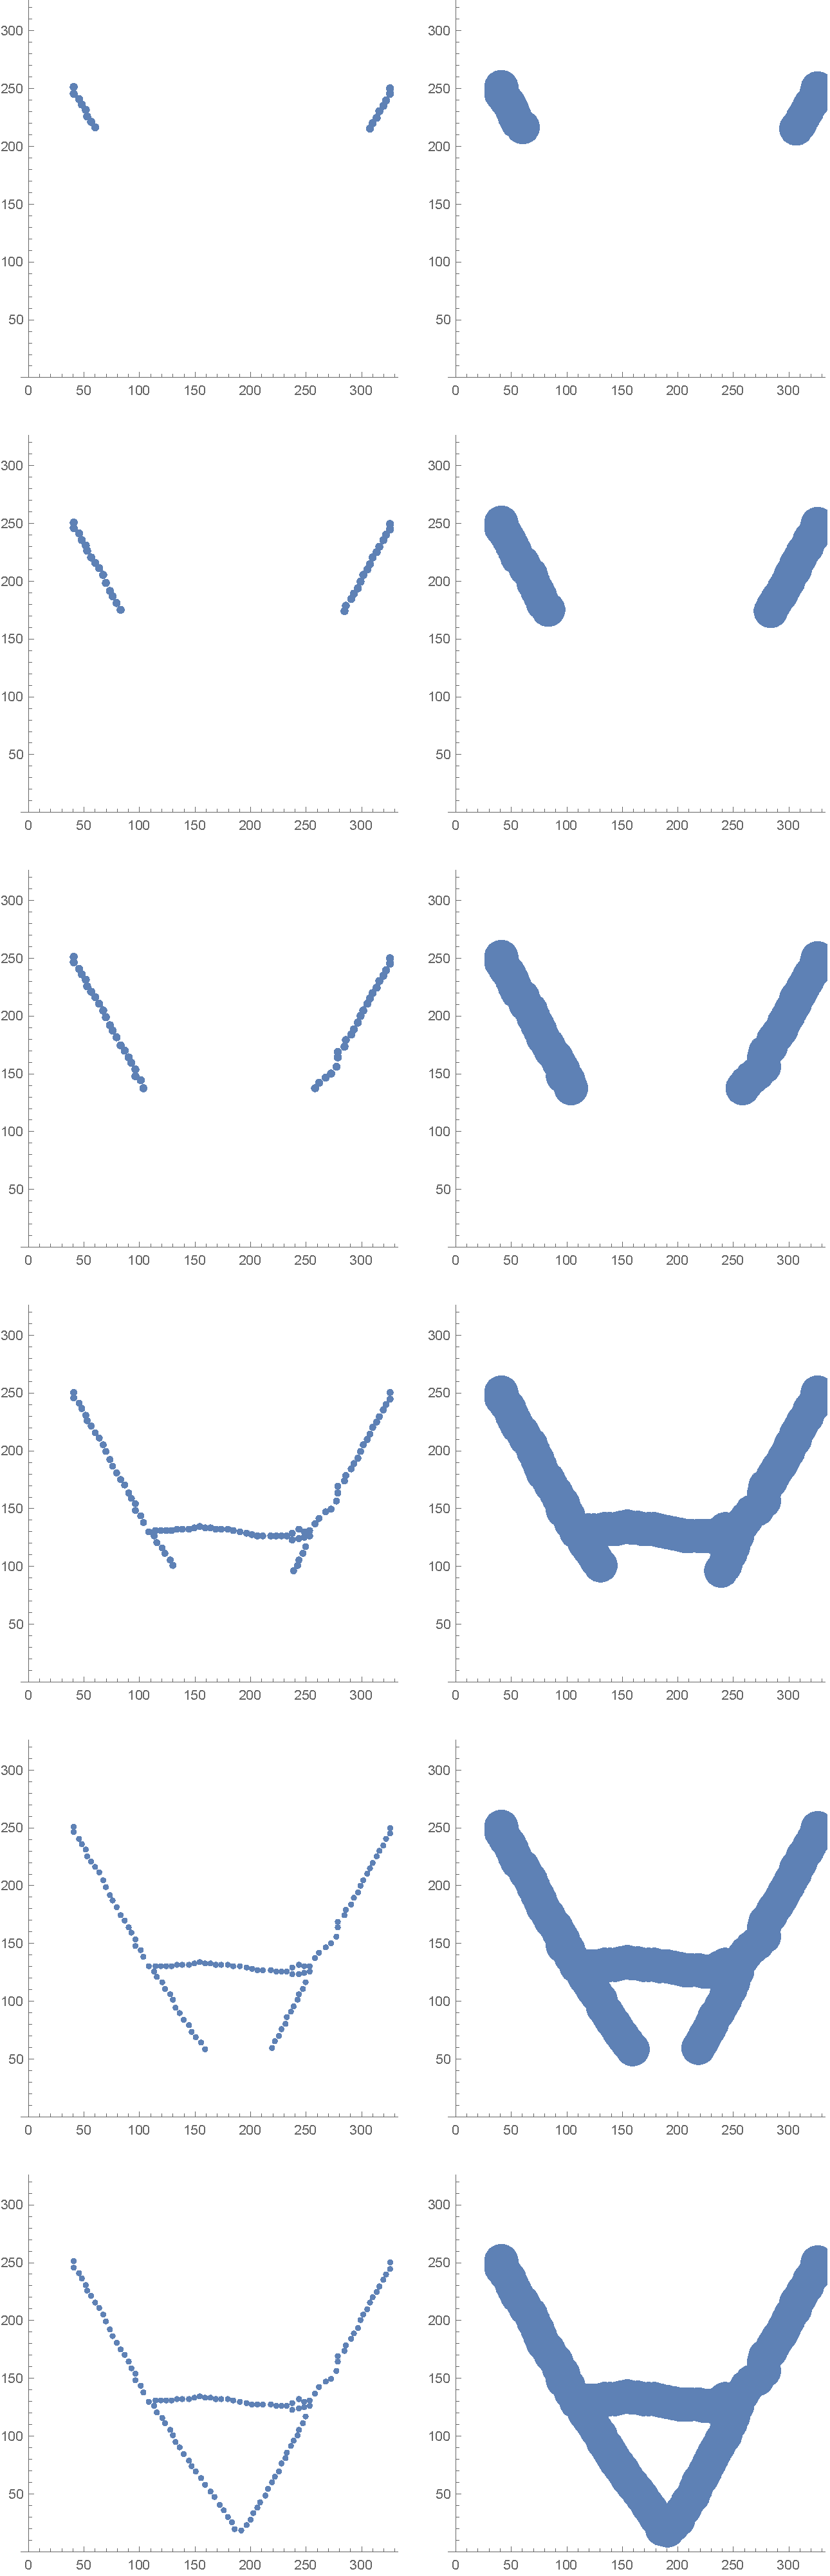
\includegraphics[scale=0.2]{../images/RT-A-cuts.pdf}
	&
	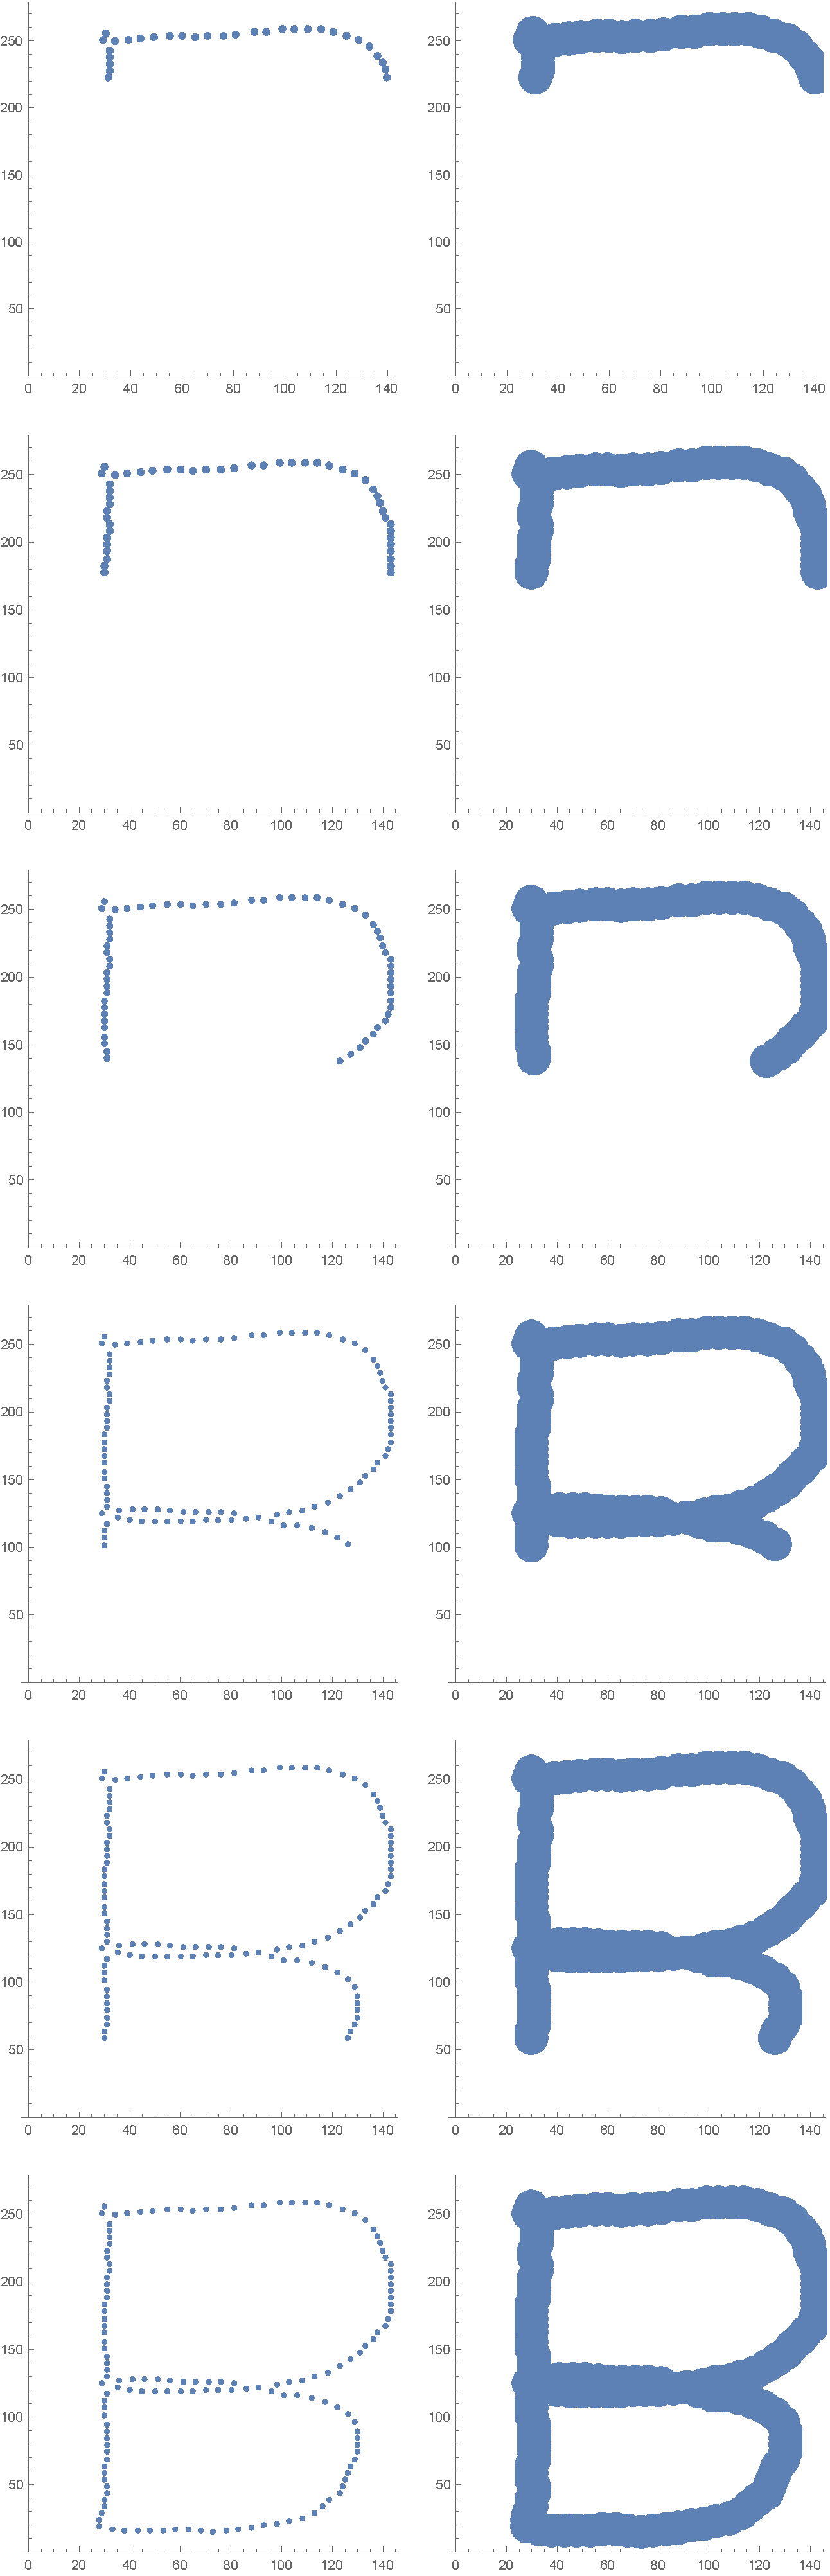
\includegraphics[scale=0.2]{../images/RT-B-cuts.pdf}
	&
	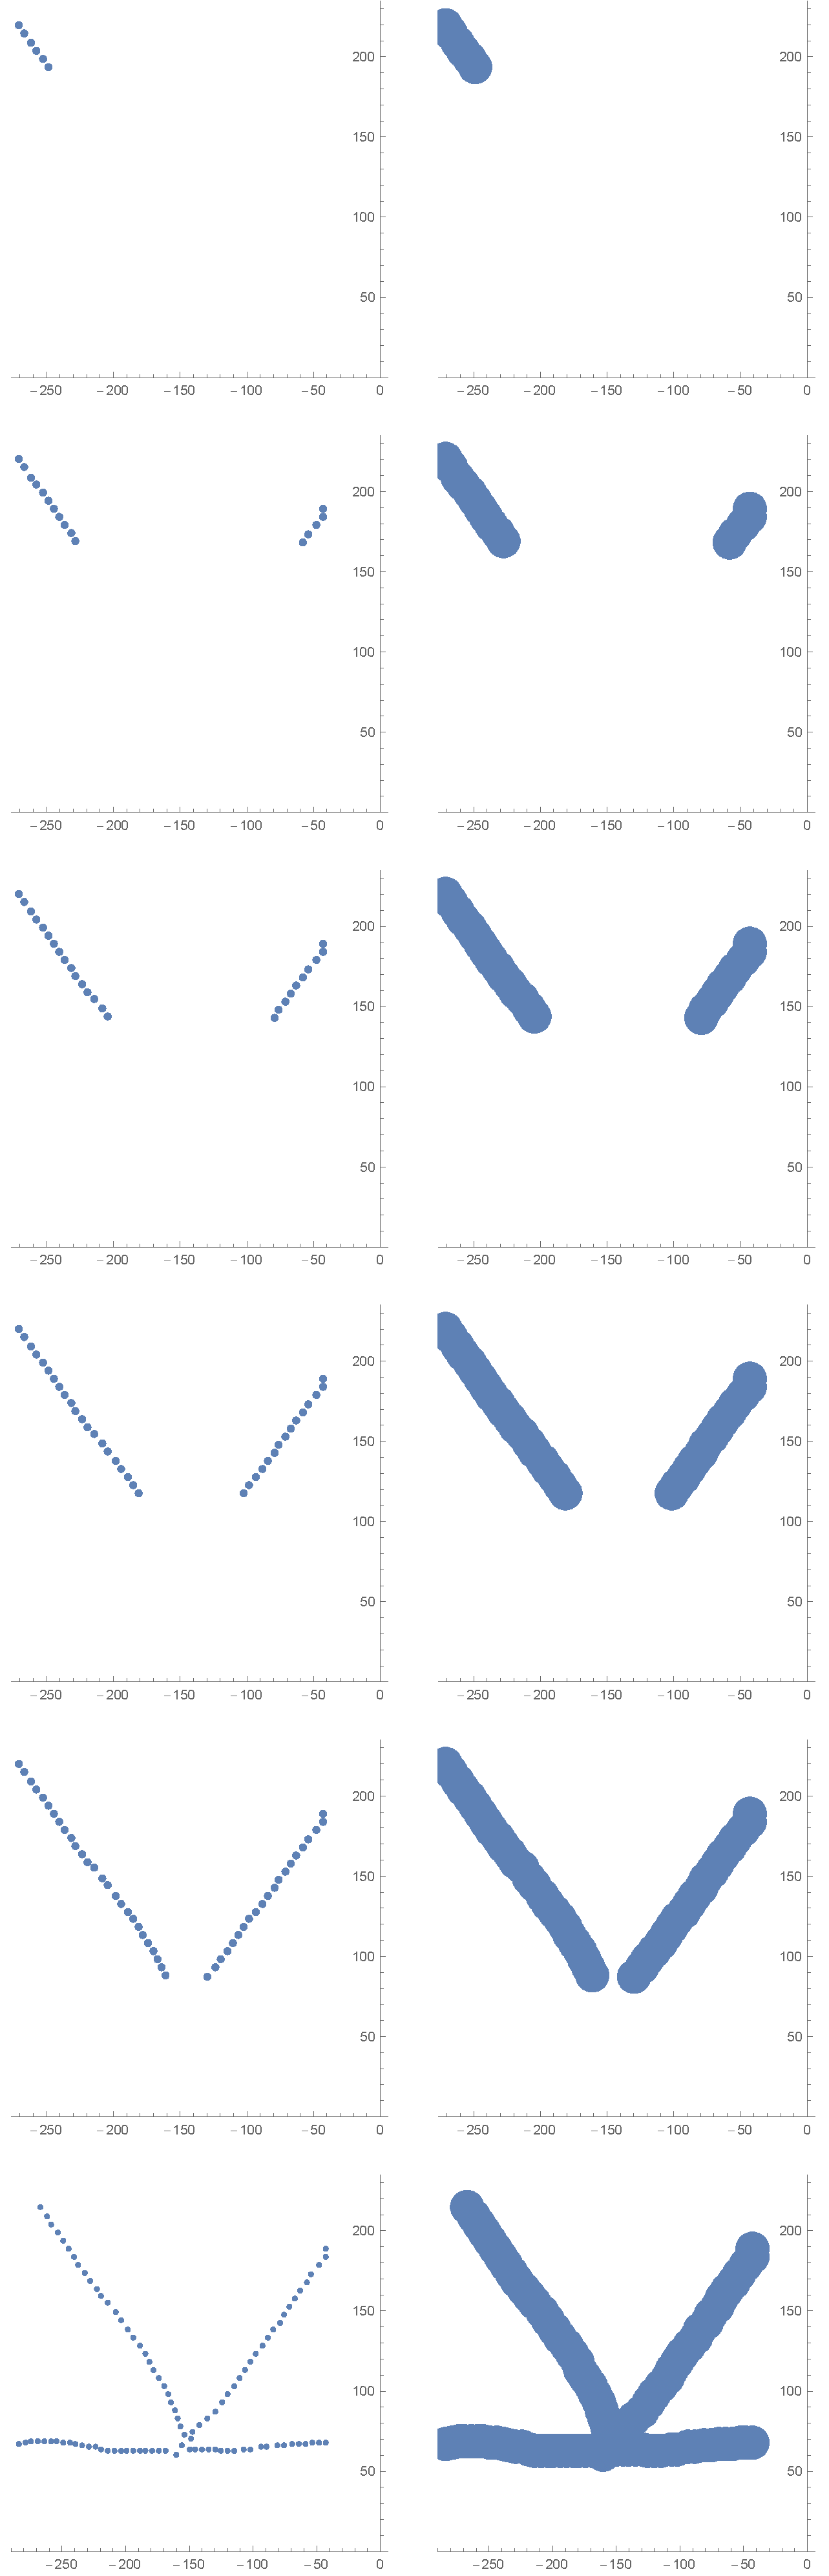
\includegraphics[scale=0.2]{../images/RT-K-90-cuts.pdf}\\
      
	\multicolumn{3}{c}{Fig 1: Sinking of letters A, B and K (rotated for 90 degrees)}
\end{tabular}

%----------------------------------------------------------------------------------------
%	SECTION 4
%----------------------------------------------------------------------------------------

\section{Results}
We were able to classify all 12 letters using only their topological properties. We used a solution that does not even need first dimension simplices from the input. We only need points (0-dimension simplices). We were successful in solving the main problem.


%----------------------------------------------------------------------------------------
%	SECTION 5
%----------------------------------------------------------------------------------------

\section{Conclusion}
\begin{itemize}
\item The biggest problem we had was to classify the letter I. The object itself is really simple but when you try to compute homology from the side, everything detected is treated as an error. Many solutions are possible, we just checked if the letter width is lower than our error margin and computed its homology as a whole.

\item The project is easily extendible to the whole alphabet. Lower case letters or special characters can easily be added. The main problem with this approach is that we need a ''pretty'' input. When the letters are ie. too close together, curved or one over the other, these topological data are not so helpful.

\item For creating Vietoris-Rips complexes and computing betti numbers we used a library for topological computations called \textit{javaplex}.
\end{itemize}


\end{document}